\documentclass{article}

\usepackage{polski}
\usepackage[utf8]{inputenc}

\usepackage[letterpaper,top=2cm,bottom=2cm,left=3cm,right=3cm,marginparwidth=1.75cm]{geometry}

% Useful packages
\usepackage{amsmath}
\usepackage{graphicx}
\usepackage[colorlinks=true, allcolors=blue]{hyperref}

% Default fixed font does not support bold face
\DeclareFixedFont{\ttb}{T1}{txtt}{bx}{n}{12} % for bold
\DeclareFixedFont{\ttm}{T1}{txtt}{m}{n}{12}  % for normal

% Custom colors
\usepackage{color}
\definecolor{deepblue}{rgb}{0,0,0.5}
\definecolor{deepred}{rgb}{0.6,0,0}
\definecolor{deepgreen}{rgb}{0,0.5,0}

\usepackage{listings}

% Python style for highlighting
\newcommand\pythonstyle{\lstset{
language=Python,
basicstyle=\ttm,
morekeywords={self},              % Add keywords here
keywordstyle=\ttb\color{deepblue},
emph={MyClass,__init__},          % Custom highlighting
emphstyle=\ttb\color{deepred},    % Custom highlighting style
stringstyle=\color{deepgreen},
frame=tb,                         % Any extra options here
showstringspaces=false
}}


% Python environment
\lstnewenvironment{python}[1][]
{
\pythonstyle
\lstset{#1}
}
{}

% Python for external files
\newcommand\pythonexternal[2][]{{
\pythonstyle
\lstinputlisting[#1]{#2}}}

% Python for inline
\newcommand\pythoninline[1]{{\pythonstyle\lstinline!#1!}}


\title{\huge Aproksymacja profilu wysokościowego}
\author{Sprawozdanie z trzeciego projektu z Metod Numerycznych. Mikołaj Nowak 184865}
\date{}

\begin{document}
\maketitle


\section{Wprowadzenie}

Tematem trzeciego projektu była implementacja metod interpolacji pozwalających na aproksymację profilów wysokościowych.
Profil wysokościowy trasy, inaczej zwany profilem topograficznym trasy, to wykres, który przedstawia bezwzględną wysokość w terenie w zależności od odległości punktu od początku trasy. Posiada to praktyczne zastosowanie w przypadku np. osób planujących wycieczkę górską.
Tematem trzeciego projektu była aproksymacja ów profilu wysokościowego z użyciem dwóch metod:
\begin{itemize}
  \item wykorzystującej wielomian interpolacyjny Lagrange'a,
  \item wykorzystującej funkcje sklejane trzeciego stopnia.
\end{itemize}
Interpolacja to nic innego jak estymacja wartości badanej wielkości w obszarach pomiędzy dyskretnymi punktami.
Jest ona szeroko wykorzystywana w uczeniu maszynowym, statystyce, systemach sensorowych itp.
Informacje o punktach pomiarowych na poszczególnych terenach zaczerpnąłem z gotowych danych dostępnych na kursie.

\section{Metody aproksymacji interpolacyjnej}

\subsection{Metoda wykorzystująca wielomian interpolacyjny Lagrange'a}
Interpolacja Lagrange'a jest przykładem interpolacji globalnej i jest tym samym dość ryzykowna co zostanie przedstawione w dalszym
etapie sprawozdania. Udoskonala ona zwykłą interpolację wielomianową poprzez znalezienie lepszej bazy funkcji do interpolacji.
W ramach implementacji tej metody skorzystałem z dwóch poniższych wzorów, które zostały przedstawione na wykładzie:
\begin{itemize}
    \item wzór na bazę do interpolacji:
    \begin{equation}
    \phi = \prod_{j=1, j \neq i}^{n+1} \dfrac{(x-x_j)}{(x_i-x_j)} \text{\space \space dla i=1, 2 ... n+1}
    \end{equation}
    \item wzór na funkcję interpolującą F(x):
    \begin{equation}
    F(x) = \sum_{i=1}^{n+1} y_i \phi_i
    \end{equation}
\end{itemize}

\newpage

Kod metody wykorzystującej wielomian interpolacyjny Lagrange'a prezentuje się następująco:

\begin{python}
def phi(vec_x, x, i, n):
    product = 1.0
    for j in range(n):
        if j == i:
            continue  # avoid diving by zero
        product *= (x-vec_x[j])/(vec_x[i]-vec_x[j])
    return product


def Lagrange_interpolation(vec_x, vec_y, x, n):
    series_sum = 0
    for i in range(n):
        series_sum += vec_y[i]*phi(vec_x, x, i, n)
    return series_sum


def Lagrange_method(name, path, delimiter, intervals_num):
    data_x, data_y = read_input(path, delimiter)
    intervals = make_intervals(0, len(data_x), intervals_num)
    vec_x = [data_x[i] for i in intervals]
    vec_y = [data_y[i] for i in intervals]
    interpol = []
    for i, x in enumerate(data_x):
        if intervals[-1] < i:
            break
        interpol.append(Lagrange_interpolation(vec_x, vec_y, x, 
                                               len(vec_x)))
    plt.plot(data_x, data_y)
    plt.plot(data_x[:intervals[-1] + 1], interpol)
    plt.plot(vec_x, vec_y, 'o')
    tmp_str = 'Lagrange interpolation, ' + name + \
              ', N = ' + str(intervals_num)
    plt.title(tmp_str)
    filename = name.replace(" ", "_")
    plt.savefig(filename + '_Lagrange_N_'+str(intervals_num)+'.png')
    plt.show()
\end{python}

\newpage

Po wywołaniu otrzymujemy następujące rezultaty:
\begin{itemize}
    
    \item dla Głębi Challengera:
    \begin{figure}[!htb]
    \minipage{0.48\textwidth}
      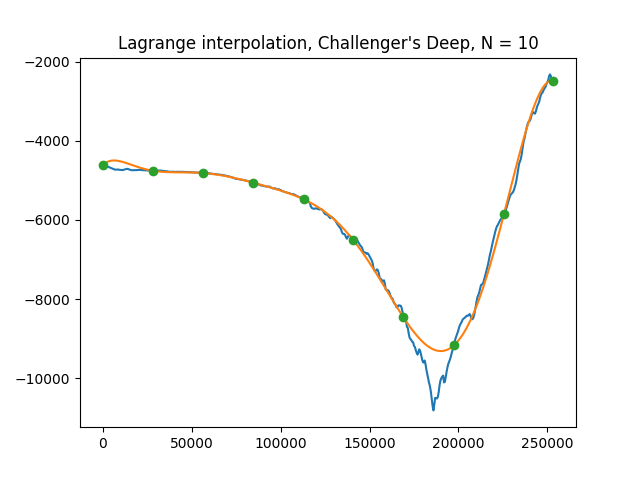
\includegraphics[width=\linewidth]{Challenger's_Deep_Lagrange_N_10.png}
      \caption{Interpolacja Lagrange'a dla N=10}
    \endminipage\hfill
    \minipage{0.48\textwidth}
      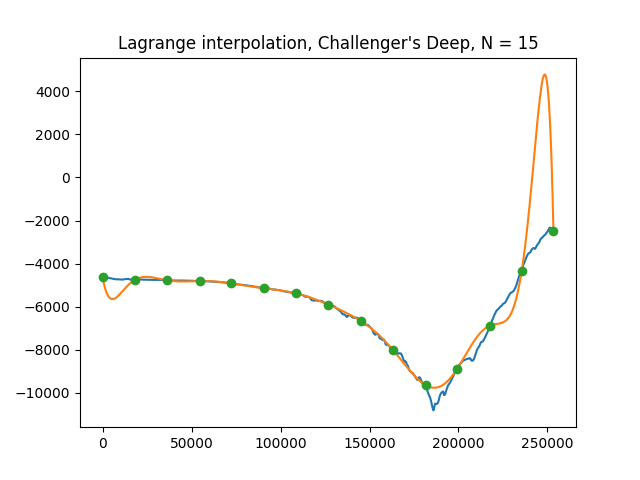
\includegraphics[width=\linewidth]{Challenger's_Deep_Lagrange_N_15.png}
      \caption{Interpolacja Lagrange'a dla N=15}
    \endminipage\hfill
    \end{figure}
    
    \item dla Wielkiego Kanionu:
    \begin{figure}[!htb]
    \minipage{0.48\textwidth}
      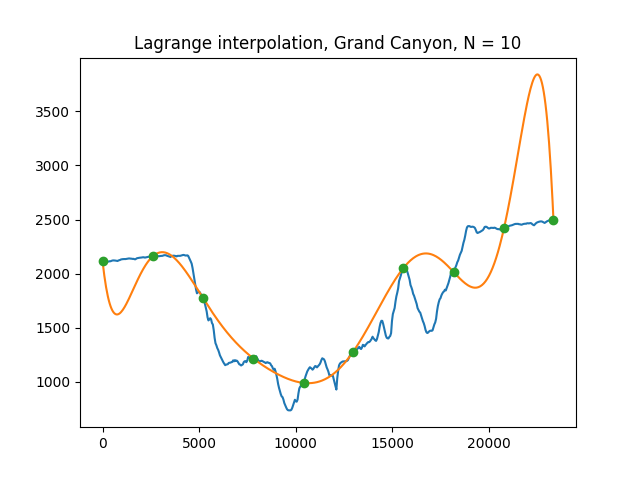
\includegraphics[width=\linewidth]{Grand_Canyon_Lagrange_N_10.png}
      \caption{Interpolacja Lagrange'a dla N=10}
    \endminipage\hfill
    \minipage{0.48\textwidth}
      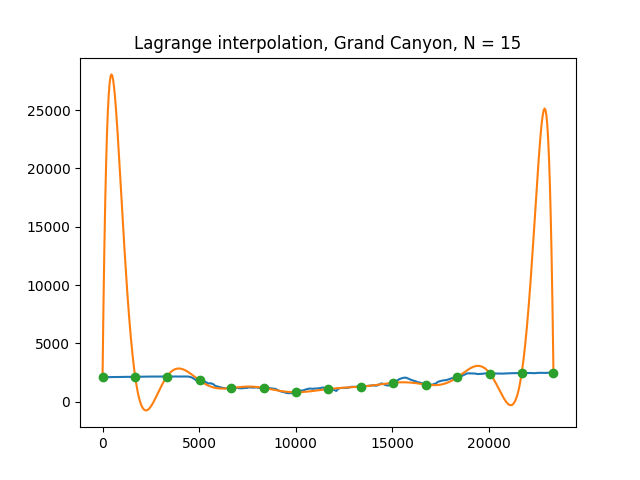
\includegraphics[width=\linewidth]{Grand_Canyon_Lagrange_N_15.png}
      \caption{Interpolacja Lagrange'a dla N=15}
    \endminipage\hfill
    \end{figure}  
    
    \newpage
    \item dla Trzewa oraz Starogardu:
    \begin{figure}[!htb]
    \minipage{0.48\textwidth}
      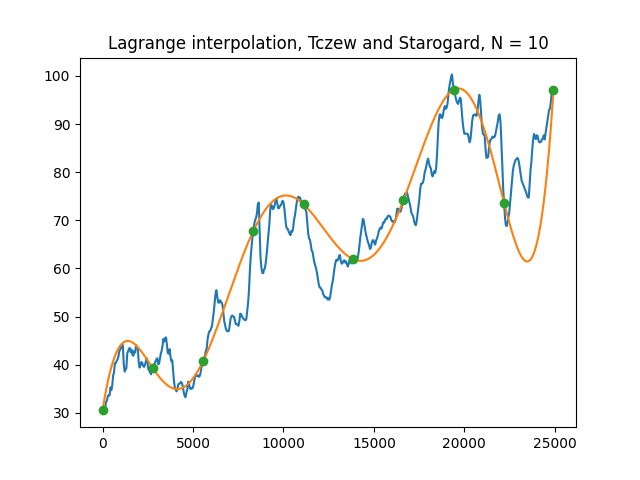
\includegraphics[width=\linewidth]{Tczew_and_Starogard_Lagrange_N_10.png}
      \caption{Interpolacja Lagrange'a dla N=10}
    \endminipage\hfill
    \minipage{0.48\textwidth}
      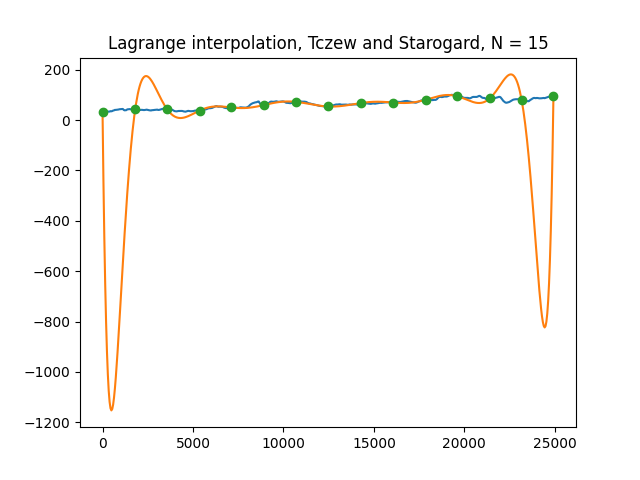
\includegraphics[width=\linewidth]{Tczew_and_Starogard_Lagrange_N_15.png}
      \caption{Interpolacja Lagrange'a dla N=15}
    \endminipage\hfill
    \end{figure}
    
    \item dla Mount Everest:
    \begin{figure}[!htb]
    \minipage{0.48\textwidth}
      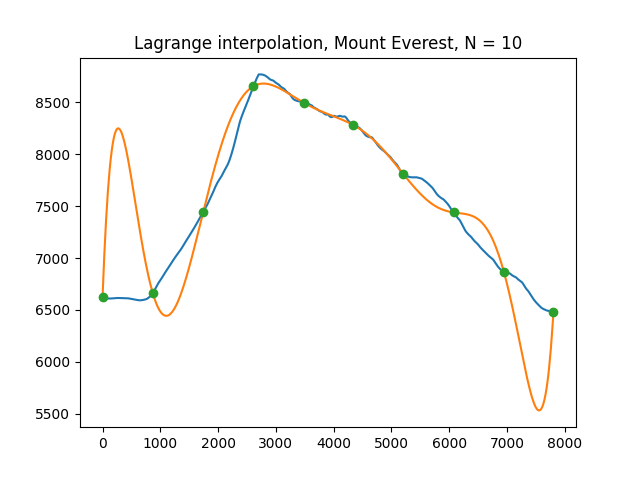
\includegraphics[width=\linewidth]{Mount_Everest_Lagrange_N_10.png}
      \caption{Interpolacja Lagrange'a dla N=10}
    \endminipage\hfill
    \minipage{0.48\textwidth}
      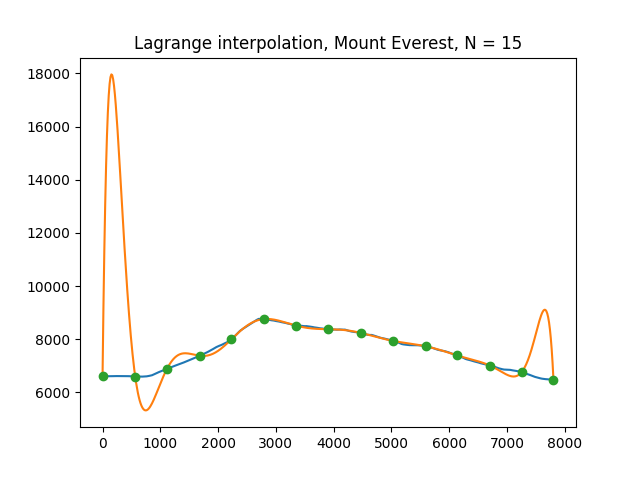
\includegraphics[width=\linewidth]{Mount_Everest_Lagrange_N_15.png}
      \caption{Interpolacja Lagrange'a dla N=15}
    \endminipage\hfill
    \end{figure}
    
\end{itemize}

Jak nietrudno zauważyć na krańcach wykresów widoczne są duże oscylacje które rosną wraz ze wzrostem ilości interpolowanych punktów i mogą
wręcz zniekształcać oryginalny wykres powstały z punktów pomiarowych. Przyczyny takiego stanu rzeczy zostaną szerzej opisane we wnioskach.

\newpage

\subsection{Metoda wykorzystująca funkcje sklejane trzeciego stopnia}

Metoda ta w odróżnieniu od metody Lagrange'a nie jest globalna, wykorzystuje interpolację lokalną (między poszczególnymi węzłami) z użyciem wielomianów niskiego stopnia \[S_0(x), S_1(x), S_2(x), ... S_n(x)\]
Ponieważ wykorzystanie funkcji sklejanych pierwszego i drugiego stopnia nie daje zadowalających rezultatów, należy
skorzystać z funkcji sklejanych trzeciego stopnia (tzw. kubicznych). W i-tym podprzedziale wielomian ma postać:
\[ S_i(x) = a_i + b_i(x-x_i) + c_i(x-x_i)^2 + d_i(x-x_i)^3 \]
Aby skorzystać z tej metody należy uwzględnić pewne założenia:
\begin{itemize}
    \item Zakładamy, że podprzedziały są równe, chociaż w ogólności nie muszą być: \break
        x\textsubscript{1} - x\textsubscript{0} = h, x\textsubscript{2} - x\textsubscript{1} = h,
    \item S(x\textsubscript{0}) i S(x\textsubscript{1}) są wielomianami 3 stopnia,
    \item S\textsubscript{0}(x\textsubscript{1}) = f(x\textsubscript{1}),
    \item S\textsubscript{1}(x\textsubscript{1}) = f(x\textsubscript{1}),
    \item S\textsubscript{1}(x\textsubscript{2}) = f(x\textsubscript{2}),
    \item S\textsubscript{1}(x\textsubscript{2}) = f(x\textsubscript{2}),
    \item Dla granicznego węzła ciągłość pierwszej pochodnej x\textsubscript{1},
    \item Dla granicznego węzła ciągłość drugiej pochodnej x\textsubscript{1},
    \item Na krańcach zerowanie drugej pochodnej.
\end{itemize}
Razem daje to 8 niewiadomych współczynników i 8 równań.
W ramach tej metoda wykorzystującej funkcje sklejane trzeciego stopnia skorzystałem z autorskiej implementacji macierzy z poprzedniego projektu. Kod klasy poniżej:

\begin{python}
class Matrix:
    def __init__(self, N, a1=1, a2=0, a3=0):  
        # identity matrix by default, a2 and a3 are used for 
        # band matrices
        self.N = N
        self.data = [[0 for _ in range(N)] for _ in range(N)]
        for i in range(N):
            self.data[i][i] = a1
            if i + 1 < N:
                self.data[i][i + 1] = a2
                self.data[i + 1][i] = a2
            if i + 2 < N:
                self.data[i][i + 2] = a3
                self.data[i + 2][i] = a3

    def __str__(self):
        # graphic representation of a matrix, working well only with 
        # relatively small matrices
        string = ""
        for row in self.data:
            for value in row:
                string += str(round(value, 2))
                string += "\t\t"
            string += '\n'
        return string

    def __add__(self, other):
        for i in range(self.N):
            for j in range(self.N):
                self.data[i][j] += other.data[i][j]

    def __sub__(self, other):
        for i in range(self.N):
            for j in range(self.N):
                self.data[i][j] -= other.data[i][j]

    def __mul__(self, vector):  # only matrix times vector
        vtr = [0 for _ in range(self.N)]  # vector to return
        for i in range(self.N):
            for j in range(self.N):
                vtr[i] += self.data[i][j] * vector[j]
        return vtr

    def get_copy(self):  # returns deepcopy of a matrix
        copy = Matrix(self.N)
        for i in range(self.N):
            for j in range(self.N):
                copy.data[i][j] = self.data[i][j]
        return copy
\end{python}

Z poprzedniego projektu zaczerpnąłem także metodę LU, natomiast ze względu na pojawianie się zer na głównej diagonali dodałem do niej pivoting. Kod poniżej:

\begin{python}
def find_pivot(U, i):
    pivot = abs(U.data[i][i])
    pivot_index = i
    for j in range(i+1, U.N):
        if abs(U.data[j][i] > pivot):
            pivot = abs(U.data[j][i])
            pivot_index = j
    return pivot, pivot_index


def pivoting(L, U, P, i):
    pivot, pivot_index = find_pivot(U, i)
    if pivot_index == i:
        return  # no need for interchanging rows
    for j in range(i, U.N):
        U.data[i][j], U.data[pivot_index][j] = U.data[pivot_index][j], \
        U.data[i][j]
    for j in range(i):
        L.data[i][j], L.data[pivot_index][j] = L.data[pivot_index][j], \
        L.data[i][j]
    for j in range(U.N):
        P.data[i][j], P.data[pivot_index][j] = P.data[pivot_index][j], \
        P.data[i][j]


def create_LUP_matrices(matrix):
    L = Matrix(matrix.N)
    U = matrix.get_copy()
    P = Matrix(matrix.N)  # permutation matrix
    for i in range(matrix.N-1):
        pivoting(L, U, P, i)
        for j in range(i+1, matrix.N):
            L.data[j][i] = U.data[j][i]/U.data[i][i]
            for k in range(i, matrix.N):
                U.data[j][k] -= L.data[j][i]*U.data[i][k]
    return L, U, P


def norm(vec):
    N = len(vec)
    n = 0  # norm
    for i in range(N):
        n += vec[i]**2
    return math.sqrt(n)


def residual(matrix, vec_x, vec_b):
    N = len(vec_x)
    product = matrix*vec_x
    res = [(product[i] - vec_b[i]) for i in range(N)]
    return res


def LU_decomposition(A, b):  # with pivoting
    x = [0 for _ in range(A.N)]
    y = [0 for _ in range(A.N)]
    L, U, P = create_LUP_matrices(A)
    b = P*b
    for i in range(A.N):
        series_sum = 0
        for j in range(i):
            series_sum += L.data[i][j]*y[j]
        y[i] = (b[i] - series_sum)
    for i in range(A.N-1, -1, -1):
        series_sum = 0
        for j in range(i+1, A.N):
            series_sum += U.data[i][j] * x[j]
        x[i] = (y[i] - series_sum)/U.data[i][i]
    res = residual(A, x, b)
    return x, y, norm(res)
\end{python}

\newpage
Najważniejszy aspekt, czyli metody odpowiedzialne za interpolacje prezentują się następująco:

\begin{python}
def spline_interpolation(vec_x, vec_y, n):
    intervals_number = len(vec_x) - 1
    size = intervals_number * 4  # due to 4 factors (a,b,c,d)
    A = Matrix(size, 0)
    b = [0 for i in range(size)]
    h = (vec_x[-1]-vec_x[0])/intervals_number  
    # Assuming that intervals are equal

    for i in range(0, intervals_number):
        A.data[2*i][4*i] = 1
        A.data[2*i + 1][4*i], A.data[2*i + 1][4*i + 1] = 1, h
        A.data[2*i + 1][4*i + 2], A.data[2*i + 1][4*i + 3] = h**2, h**3
        if i < intervals_number-1:
            A.data[i * 2 + intervals_number*2][4 * i + 1] = 1
            A.data[i * 2 + intervals_number*2][4 * i + 2] = 2 * h
            A.data[i * 2 + intervals_number*2][4 * i + 3] = 3 * (h ** 2)
            A.data[i * 2 + intervals_number*2][4 * i + 5] = -1
            A.data[i * 2 + intervals_number*2 + 1][4 * i + 2] = 2
            A.data[i * 2 + intervals_number*2 + 1][4 * i + 3] = 6 * h
            A.data[i * 2 + intervals_number*2 + 1][4 * i + 6] = -2
        b[2 * i], b[2 * i + 1] = vec_y[i], vec_y[i + 1]
    A.data[-1][-2], A.data[-1][-1] = 2, 6 * h
    A.data[-2][2] = 2

    lux, _, _ = LU_decomposition(A, b)  # LU decomposition with pivoting

    results_x, results_y = [], []
    for i in range(0, intervals_number):
        dx = make_intervals(vec_x[0] + i * h, vec_x[0] + (i + 1) * h, \
                            n//size)
        a, b, c, d = lux[4*i], lux[4*i+1], lux[4*i+2], lux[4*i+3]
        beg = (vec_x[0]+i*h)
        dy = [(d * (x - beg)**3 + c * (x - beg)**2 + b * (x - beg) + \
               a) for x in dx] 
        results_x += dx
        results_y += dy

    return results_x, results_y


def splines_method(name, path, delimiter, intervals_num):
    data_x, data_y = read_input(path, delimiter)
    intervals = make_intervals(0, len(data_x), intervals_num)
    vec_x = [data_x[i] for i in intervals]
    vec_y = [data_y[i] for i in intervals]
    result_x, result_y = spline_interpolation(vec_x, vec_y, 
                                              intervals_num*100)
    plt.plot(data_x, data_y)
    plt.plot(result_x, result_y)
    plt.plot(vec_x, vec_y, 'o')
    tmp_str = 'Spline interpolation, ' + name + ', N = ' + \
               str(intervals_num)
    plt.title(tmp_str)
    filename = name.replace(" ", "_")
    plt.savefig(filename + '_splines_N_' + str(intervals_num) + '.png')
    plt.show()
\end{python}

Poniżej rezultat wykonania metody wykorzystującej funkcje sklejane trzeciego stopnia:

Po wywołaniu otrzymujemy następujące rezultaty:
\begin{itemize}
    
    \item dla Głębi Challengera:
    \begin{figure}[!htb]
    \minipage{0.32\textwidth}
      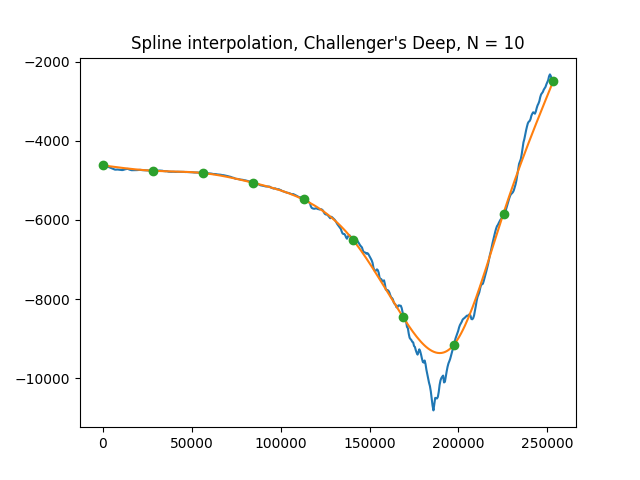
\includegraphics[width=\linewidth]{Challenger's_Deep_splines_N_10.png}
      \caption{Interpolacja przy użyciu funkcji sklejanych dla N=10}
    \endminipage\hfill
    \minipage{0.32\textwidth}
      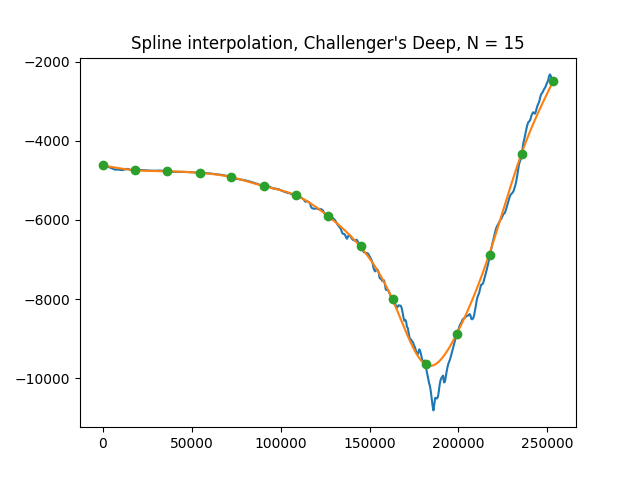
\includegraphics[width=\linewidth]{Challenger's_Deep_splines_N_15.png}
      \caption{Interpolacja przy użyciu funkcji sklejanych dla N=15}
    \endminipage\hfill
    \minipage{0.32\textwidth}
      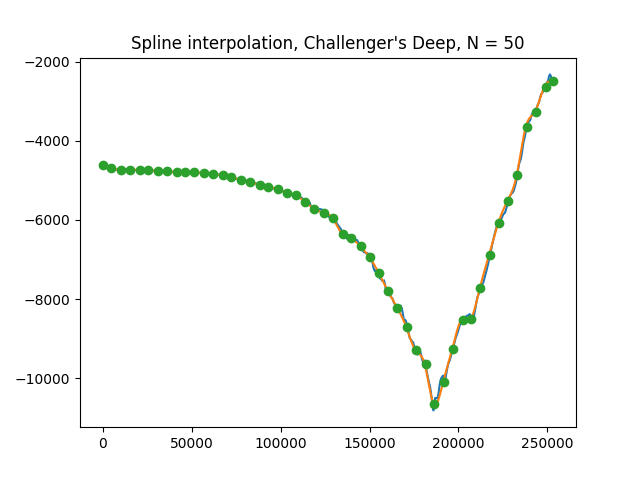
\includegraphics[width=\linewidth]{Challenger's_Deep_splines_N_50.png}
      \caption{Interpolacja przy użyciu funkcji sklejanych dla N=50}
    \endminipage\hfill
    \end{figure}
    
    \item dla Wielkiego Kanionu:
    \begin{figure}[!htb]
    \minipage{0.32\textwidth}
      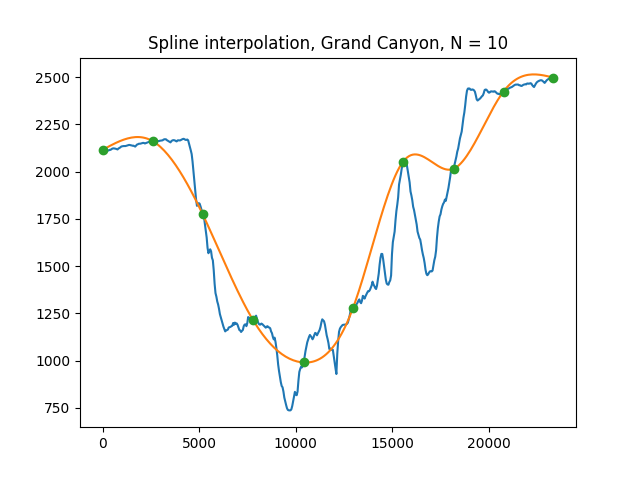
\includegraphics[width=\linewidth]{Grand_Canyon_splines_N_10.png}
      \caption{Interpolacja przy użyciu funkcji sklejanych dla N=10}
    \endminipage\hfill
    \minipage{0.32\textwidth}
      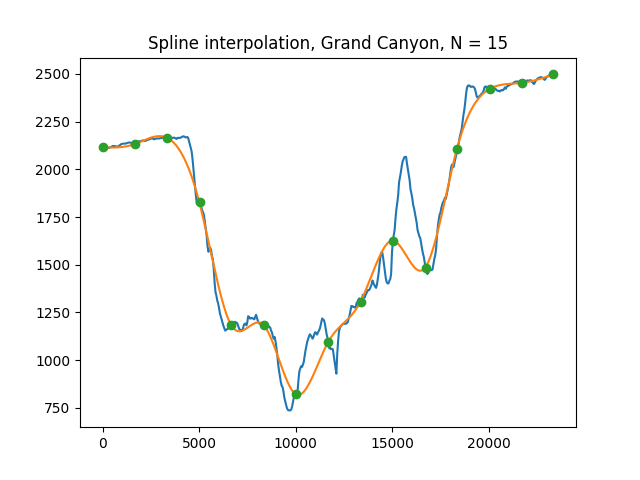
\includegraphics[width=\linewidth]{Grand_Canyon_splines_N_15.png}
      \caption{Interpolacja przy użyciu funkcji sklejanych dla N=15}
    \endminipage\hfill
    \minipage{0.32\textwidth}
      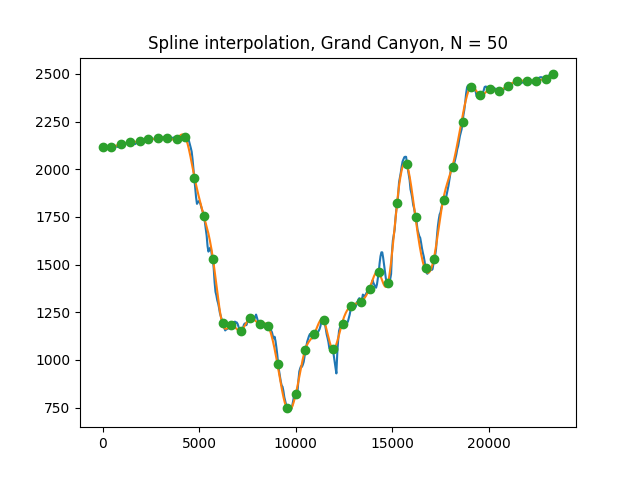
\includegraphics[width=\linewidth]{Grand_Canyon_splines_N_50.png}
      \caption{Interpolacja przy użyciu funkcji sklejanych dla N=50}
    \endminipage\hfill
    \end{figure}
    
    \newpage
    \item dla Trzewa oraz Starogardu:
    \begin{figure}[!htb]
    \minipage{0.32\textwidth}
      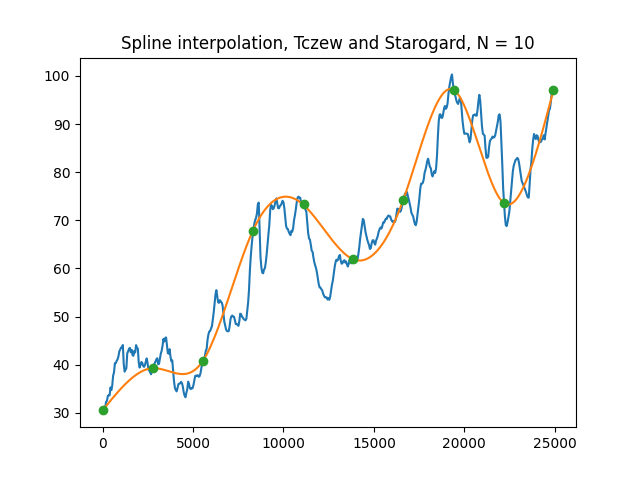
\includegraphics[width=\linewidth]{Tczew_and_Starogard_splines_N_10.png}
      \caption{Interpolacja przy użyciu funkcji sklejanych dla N=10}
    \endminipage\hfill
    \minipage{0.32\textwidth}
      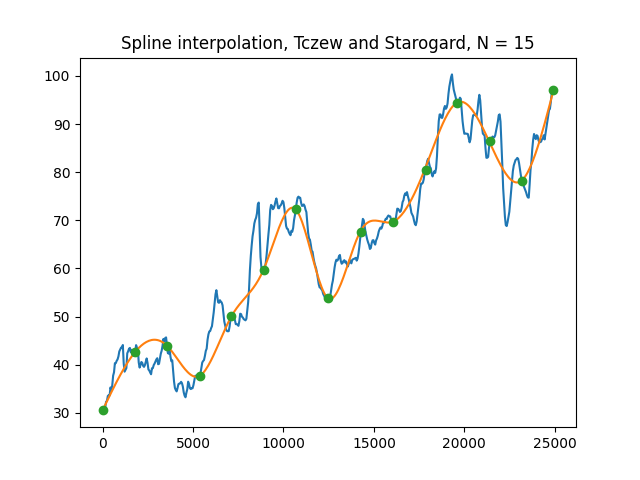
\includegraphics[width=\linewidth]{Tczew_and_Starogard_splines_N_15.png}
      \caption{Interpolacja przy użyciu funkcji sklejanych dla N=15}
    \endminipage\hfill
    \minipage{0.32\textwidth}
      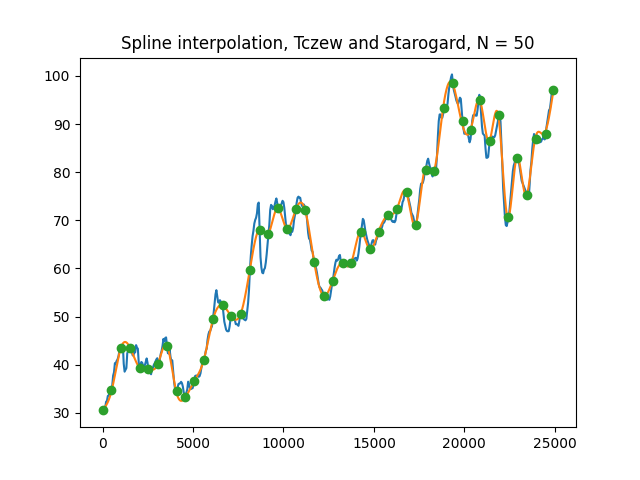
\includegraphics[width=\linewidth]{Tczew_and_Starogard_splines_N_50.png}
      \caption{Interpolacja przy użyciu funkcji sklejanych dla N=50}
    \endminipage\hfill
    \end{figure}
    
    \item dla Mount Everest:
    \begin{figure}[!htb]
    \minipage{0.32\textwidth}
      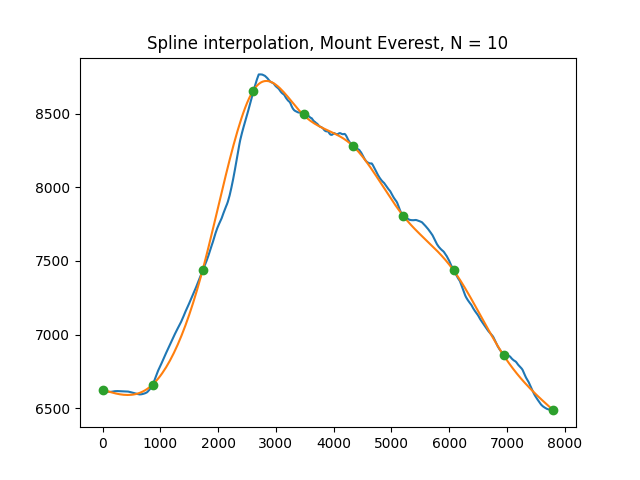
\includegraphics[width=\linewidth]{Mount_Everest_splines_N_10.png}
      \caption{Interpolacja przy użyciu funkcji sklejanych dla N=10}
    \endminipage\hfill
    \minipage{0.32\textwidth}
      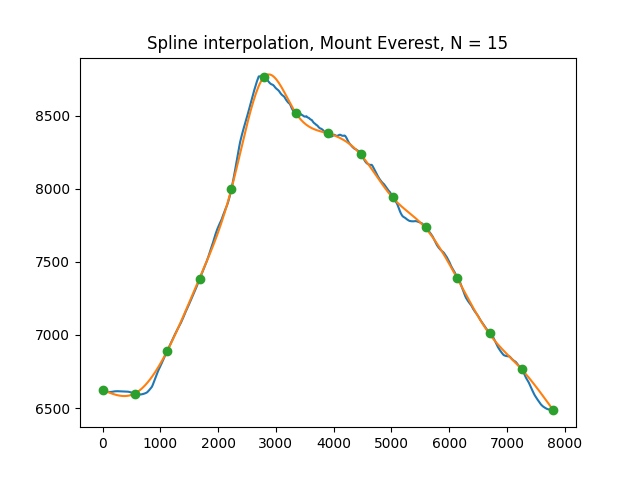
\includegraphics[width=\linewidth]{Mount_Everest_splines_N_15.png}
      \caption{Interpolacja przy użyciu funkcji sklejanych dla N=15}
    \endminipage\hfill
    \minipage{0.32\textwidth}
      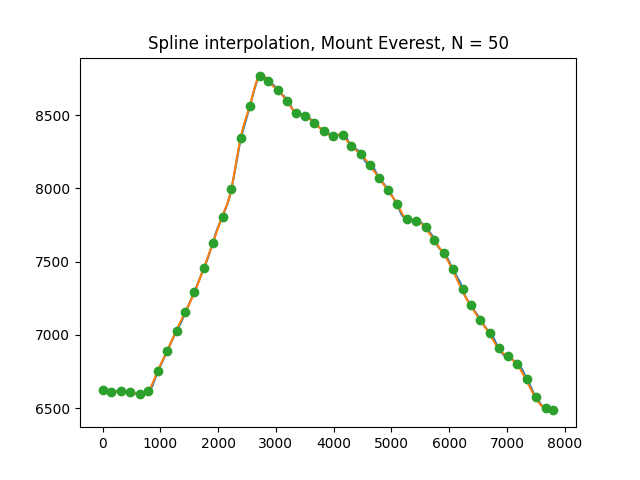
\includegraphics[width=\linewidth]{Mount_Everest_splines_N_50.png}
      \caption{Interpolacja przy użyciu funkcji sklejanych dla N=50}
    \endminipage\hfill
    \end{figure}
    
\end{itemize}

\section{Wnioski}
Metoda wykorzystująca funkcje sklejane trzeciego stopnia dokładniej aproksymuje profil wysokościowy aniżeli metoda wykorzystująca wielomian interpolacyjny Lagrange'a, natomiast jest nieco bardziej skomplikowana obliczeniowo i wymaga rozwiązania równania macierzowego. Jej dokładność wzrasta wraz z ilością węzłów, co jest całkiem intuicyjne. Nieintuicyjnie natomiast zachowuje się metoda Lagrange'a, przy której co prawda interpolacja w środku wykresu jest dobrej jakości, natomiast w miarę zwiększania się ilości węzłów znacznie zwiększają się oscylacje na końcach przedziału. Nazywa się to tzw. efektem Rungego. Pojawia się on kiedy wykorzystuje się wielomiany wysokiego stopnia do interpolacji węzłów w równo-odległych punktach. Istnieją sposoby na omijanie tego efektu, np. korzystanie z interpolacji za pomocą funkcji Czebyszewa. Przez wzgląd na fakt, iż w przypadku interpolacji globalnych, takich jak np. metoda Lagrange'a zbyt duża ilość węzłów powoduje efekt Rungego, a zbyt mała niedokładną interpolację, możemy wysnuć wniosek, iż jest ona ryzykowna. Rozsądniejszym wyborem jest skorzystanie z interpolacji lokalnej jak w przypadku wyżej opisanej metody wykorzystującej funkcje sklejane trzeciego stopnia.

\end{document}